\documentclass[preprint,12pt]{elsarticle}

%% Use the option review to obtain double line spacing
%% \documentclass[preprint,review,12pt]{elsarticle}

%% Use the options 1p,twocolumn; 3p; 3p,twocolumn; 5p; or 5p,twocolumn
%% for a journal layout:
%% \documentclass[final,1p,times]{elsarticle}
%% \documentclass[final,1p,times,twocolumn]{elsarticle}
%% \documentclass[final,3p,times]{elsarticle}
%% \documentclass[final,3p,times,twocolumn]{elsarticle}
%% \documentclass[final,5p,times]{elsarticle}
%% \documentclass[final,5p,times,twocolumn]{elsarticle}

%% The graphicx package provides the includegraphics command.
\usepackage{graphicx}
%% The amssymb package provides various useful mathematical symbols
\usepackage{amssymb}
%% The amsthm package provides extended theorem environments
%% \usepackage{amsthm}

%% The lineno packages adds line numbers. Start line numbering with
%% \begin{linenumbers}, end it with \end{linenumbers}. Or switch it on
%% for the whole article with \linenumbers after \end{frontmatter}.
\usepackage{lineno}

%% natbib.sty is loaded by default. However, natbib options can be
%% provided with \biboptions{...} command. Following options are
%% valid:

%%   round  -  round parentheses are used (default)
%%   square -  square brackets are used   [option]
%%   curly  -  curly braces are used      {option}
%%   angle  -  angle brackets are used    <option>
%%   semicolon  -  multiple citations separated by semi-colon
%%   colon  - same as semicolon, an earlier confusion
%%   comma  -  separated by comma
%%   numbers-  selects numerical citations
%%   super  -  numerical citations as superscripts
%%   sort   -  sorts multiple citations according to order in ref. list
%%   sort&compress   -  like sort, but also compresses numerical citations
%%   compress - compresses without sorting
%%
%% \biboptions{comma,round}

% \biboptions{}

\makeatletter
\def\ps@pprintTitle{%
   \let\@oddhead\@empty
   \let\@evenhead\@empty
   \let\@oddfoot\@empty
   \let\@evenfoot\@oddfoot
}
\makeatother

\begin{document}

\begin{frontmatter}

%% Title, authors and addresses

\title{\textbf{Milestone Report} \protect\\ Estimating expected return \protect\\ of a peer-to-peer lending portfolio}

%% use the tnoteref command within \title for footnotes;
%% use the tnotetext command for the associated footnote;
%% use the fnref command within \author or \address for footnotes;
%% use the fntext command for the associated footnote;
%% use the corref command within \author for corresponding author footnotes;
%% use the cortext command for the associated footnote;
%% use the ead command for the email address,
%% and the form \ead[url] for the home page:
%%
%% \title{Title\tnoteref{label1}}
%% \tnotetext[label1]{}
%% \author{Name\corref{cor1}\fnref{label2}}
%% \ead{email address}
%% \ead[url]{home page}
%% \fntext[label2]{}
%% \cortext[cor1]{}
%% \address{Address\fnref{label3}}
%% \fntext[label3]{}


%% use optional labels to link authors explicitly to addresses:
%% \author[label1,label2]{<author name>}
%% \address[label1]{<address>}
%% \address[label2]{<address>}

\author{Zbigniew Czapran}

\address{London, United Kingdom}

\begin{keyword}
Peer-To-Peer Lending \sep Portfolio Analysis \sep Risk \sep Fintech
\end{keyword}

\end{frontmatter}

%%
%% Start line numbering here if you want
%%
%%\linenumbers

%% main text
\section{Introduction to the problem}
\label{S:1}

\subsection{Plan}

The plan is to analyse a P2P lending platform's loan book in order to predict (estimate) expected return of a loan portfolio. Analysis is performed on Bondora loan book (provided for download on their website), but the approach should be generic enough to apply to other platform's loan books.

\subsection{Client}

The client is either a sophisticated individual investor or an instutional investor. The client may hold a loan portfolio with the P2P lending platform or is planning to. Based on the analysis the client may decide how to build the portfolio or modify it (by selling part of it or buying more loans) in order to maximize the profit.

\section{Description of data}
\label{S:2}

\subsection{Data cleaning}
Bondora (on their website) publicly provides loan and historic payments data for download in a CSV format. Initially, the aim of the project is to focus on loan book and leave out historic payments data for future analysis. All loans listed earlier than 2013 have been removed from the analysis as 2013 is the first year the platform started to issue loans on an industrial scale. Additionally, only loans with status \textit{Repaid} are being considered as analysis of \textit{Current} and \textit{Late} loans without detailed look at the repayment schedule won't provide enough information to asses expected return. This filtering gives a sample size of 7167 loans with 112 features.

\begin{figure}[h]
\centering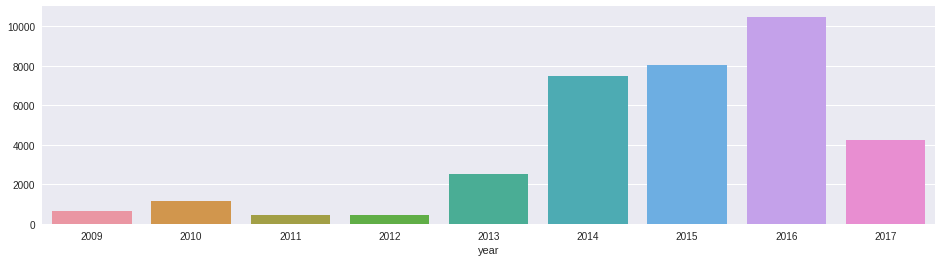
\includegraphics[width=1.0\linewidth]{plots/loans_per_year}
\caption{Number of loans per year}
\end{figure}

\subsection{Important fields}

After taking an initial look at the data, the most important fields seem to be those directly describing the contract terms (i.e. Interest Rate, Loan Amount, Loan Duration, etc.) and, secondarily, the borrower's features (i.e. Total Income, Home Ownership Type, Debt To Income Ratio, Country, Work Experience, etc.). Bondora also provides borrower's Credit Rating built on their proprietary model, although the model has changed seven times already, and renders it hard to generalise without detailed description of applied models.

\subsection{Limitations}

Because most of the loans have been originated in the recent 3 years, the number of repaid loans with durations of 48 and 60 months is significantly lower than loans of shorter duration. This will potentially create disproportion of the accuracy in the final expected return estimate depending on loan duration. Extending the analysis to include \textit{Current} and \textit{Late} loans as well as combining with historic payments, could potentially enhance accuracy for longer term loans. 

\begin{figure}[h]
\centering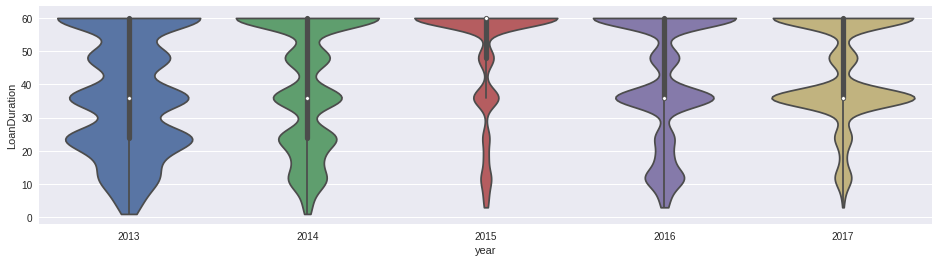
\includegraphics[width=1.0\linewidth,height=0.25\textheight]{plots/loan_duration_vs_issue_year}
\caption{Loan duration with relation to year of issue (All statuses)}
\centering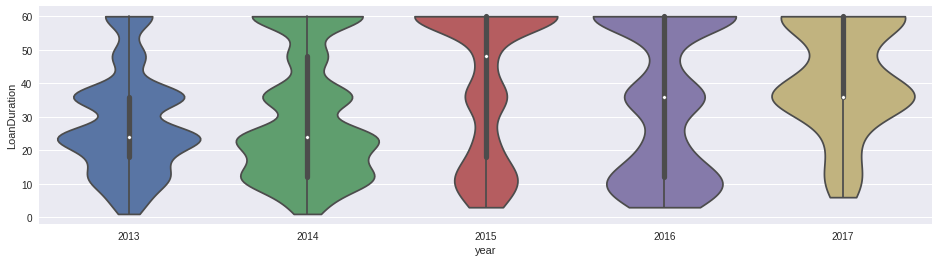
\includegraphics[width=1.0\linewidth,height=0.25\textheight]{plots/loan_duration_vs_issue_year_repaid}
\caption{Loan duration with relation to year of issue (Repaid only)}
\end{figure}

\subsection{Repayment history}

The overall default rate (loan principal hasn't been recovered fully) is \textbf{2.93\%}, the rate of recovered principal is \textbf{98.6\%}, the average interest rate paid over lifetime of a loan is \textbf{24\%}. All this gives a return of \textbf{22.6\%} for a portfolio build of all loans issued by Bondora.

\section{Exploratory Analysis}

\subsection{Analysis of impact of gender on loan features}



\begin{table}[h]
\centering
\begin{tabular}{l l l}
\hline
\textbf{Treatments} & \textbf{Response 1} & \textbf{Response 2}\\
\hline
Treatment 1 & 0.0003262 & 0.562 \\
Treatment 2 & 0.0015681 & 0.910 \\
Treatment 3 & 0.0009271 & 0.296 \\
\hline
\end{tabular}
\caption{Table caption}
\end{table}


%% The Appendices part is started with the command \appendix;
%% appendix sections are then done as normal sections
%% \appendix

%% \section{}
%% \label{}

%% References
%%
%% Following citation commands can be used in the body text:
%% Usage of \cite is as follows:
%%   \cite{key}          ==>>  [#]
%%   \cite[chap. 2]{key} ==>>  [#, chap. 2]
%%   \citet{key}         ==>>  Author [#]

%% References with bibTeX database:

\bibliographystyle{model1-num-names}
\bibliography{sample.bib}

%% Authors are advised to submit their bibtex database files. They are
%% requested to list a bibtex style file in the manuscript if they do
%% not want to use model1-num-names.bst.

%% References without bibTeX database:

% \begin{thebibliography}{00}

%% \bibitem must have the following form:
%%   \bibitem{key}...
%%

% \bibitem{}

% \end{thebibliography}

\begin{equation}
\label{eq:emc}
e = mc^2
\end{equation}

\begin{figure}[h]
\centering\includegraphics[width=0.4\linewidth]{placeholder}
\caption{Figure caption}
\end{figure}


\begin{table}[h]
\centering
\begin{tabular}{l l l}
\hline
\textbf{Treatments} & \textbf{Response 1} & \textbf{Response 2}\\
\hline
Treatment 1 & 0.0003262 & 0.562 \\
Treatment 2 & 0.0015681 & 0.910 \\
Treatment 3 & 0.0009271 & 0.296 \\
\hline
\end{tabular}
\caption{Table caption}
\end{table}



\end{document}

%%
%% End of file `elsarticle-template-1-num.tex'.